%http://www.imn.htwk-leipzig.de/~schwarz/lehre/ss17/dbv/projekte-ss17.pdf

\chapter{Programmfunktion}\label{sec:Einleitung}
Das vorliegende ImageJ-Plugin Flowig dient zur Erkennung der Bewegung eines markierten Objektes in Bildfolgen. Es wird für jedes Bild die Bewegung des Objekts im Vergleich zum vorherigen Bild erkannt.

\textbf{Eingabe: } Ein Ordner, in dem sich eine Bildfolge befindet. Ist ein Objekt in einem Bild vorhanden, muss dieses durch magentafarbene~(RGB-Wert:~255,~255,~0)\\Bounding-Boxen markiert sein.


\textbf{Ausgabe: } Bewegungsrichtung und Geschwindigkeit des Objekts in jedem Bild


\textbf{Anzeige: } Bewegungsrichtungen auf jedem Bild als Overlay, Lucas Kanade?

\section{Installation}
Bibliothek JavaCV \footnote{\url{https://github.com/bytedeco/javacv}


\section{Nutzung}

In ImageJ muss über das Menü \textbf{File} $\rightarrow$ \textbf{Import} $\rightarrow$ \textbf{Image Sequence$\dots$} eine Bildfolge geöffnet werden. 

Nachdem das Plugin auf die geöffnete Bildfolge angewandt wurde, wird in der Konsole die Bewegungsrichtung, sowie die Geschwindigkeit des Objekts in jedem Bild ausgegeben.

Für jedes Bild wird zudem ein Overlay erstellt, das die Änderung der Bewegung im Vergleich zum vorherigen Bild in Form von Pfeilen darstellt. Abbildung \ref{img:bsp2} zeigt ein beispielhaftes Overlay. Dort wird die Bewegung des Objekts von Abbildung \ref{img:bsp1} zu Abbildung \ref{img:bsp2} dargestellt.

%TODO Beispielhaftes Overlay einbinden
\begin{figure}[h]
	%\hskip-1.0cm
	\centering
	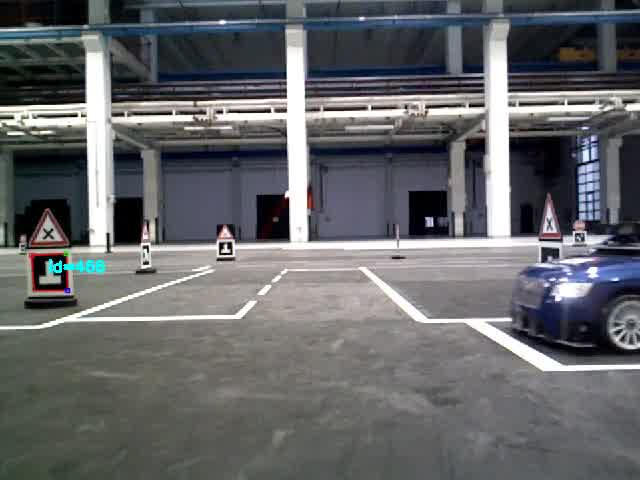
\includegraphics[scale=0.5]{./Abbildungen/bsp1.jpg}
	\caption{Beispiel 1}
	\label{img:bsp1}
\end{figure}

\begin{figure}[h]
	%\hskip-1.0cm
	\centering
	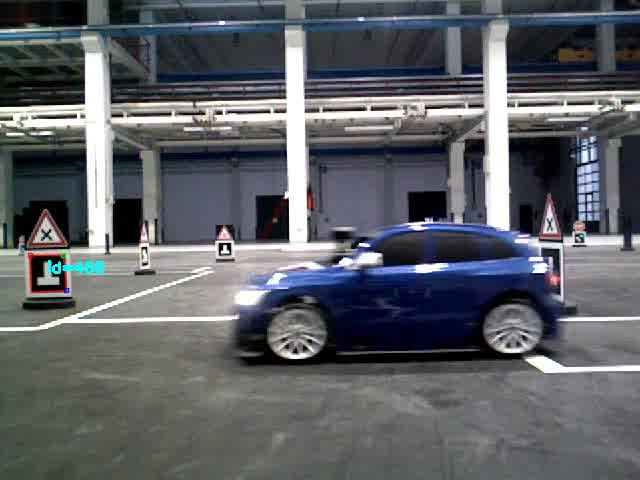
\includegraphics[scale=0.5]{./Abbildungen/bsp2.jpg}
	\caption{Bewegung zu Beispiel 1}
	\label{img:bsp2}
\end{figure}

\chapter{Bewegungserkennung}

%TODO Verfahren erläutern
In diesem Kapitel soll das genutzte Verfahren zur Erkennung von Bewegungen in Bildfolgen erläutert werden.

Das Plugin sucht zunächst nach den Bounding-Boxen. Hierzu werden alle magentafarbene Punkte der Bilder zu Bounding-Boxen zusammengefasst.

Daraufhin \dots

\chapter{title}